\begin{figure}[htbp]

      \centering
      
      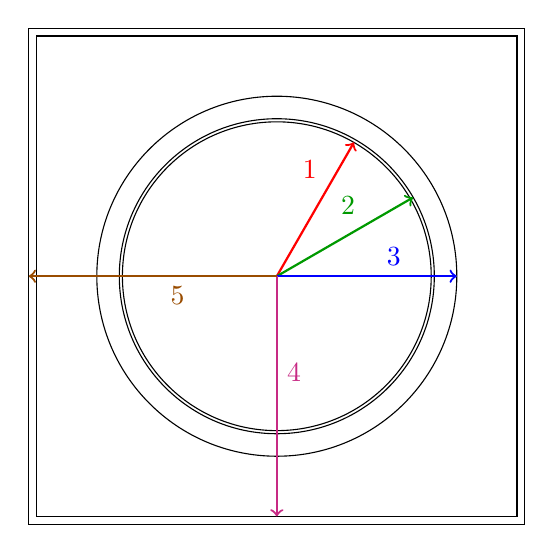
\begin{tikzpicture}[scale=5,auto]
        \draw (0,0) circle (0.39218);
      \draw[->,thick,red] (0,0) -- node[pos=0.65] {1} (0.196,0.34);
      \draw (0,0) circle (0.40005);
      \draw[->,thick,green!60!black] (0,0) -- node[pos=0.65] {2} (0.346,0.2);
      \draw (0,0) circle (0.4572);
      \draw[->,thick,blue] (0,0) -- node[pos=0.65] {3} (0.457,0.0);
      \draw (-0.61015,-0.61015) rectangle (0.61015,0.61015) ;
      \draw[->,thick,magenta!80!black] (0,0) -- node[pos=0.4] {4} (0.0,-0.61);
      \draw (-0.62992,-0.62992) rectangle (0.62992,0.62992) ;
      \draw[->,thick,orange!60!black] (0,0) -- node[pos=0.4] {5} (-0.63,0.0);

      \end{tikzpicture}
      \begin{tikzpicture}
       \matrix [matrix of nodes]
      {
          Arrow & Length (cm) & Material & \numrefheader\\
        \node[red]{1}; & \node[red]{0.39218}; & \node[red,hyperlink node=mat_fuel16]{Fuel}; & \node[red]{\ref{num:fuelpellrad}};\\ 
        \node[green!60!black]{2}; & \node[green!60!black]{0.40005}; & \node[green!60!black,hyperlink node=mat_helium]{Helium}; & \node[green!60!black]{\ref{num:fuelIRrad}};\\ 
        \node[blue]{3}; & \node[blue]{0.45720}; & \node[blue,hyperlink node=mat_zirc]{Zircaloy}; & \node[blue]{\ref{num:fuelORrad}};\\ 
        \node[magenta!80!black]{4}; & \node[magenta!80!black]{0.61015}; & \node[magenta!80!black,hyperlink node=mat_water]{Water}; & \node[magenta!80!black]{\ref{num:grid_spacer}};\\ 
        \node[orange!60!black]{5}; & \node[orange!60!black]{0.62992}; & \node[orange!60!black,hyperlink node=mat_inconel]{Inconel}; & \node[orange!60!black]{\ref{num:grid_spacer}};\\ 
      };
      \end{tikzpicture}

      \caption[Fuel pincell geometry for the top/bottom grid spacer inner egg-crate]{ Fuel pincell geometry for the Inconel 718 top/bottom grid spacer inner egg-crate, chosen to have a thickness of 0.0198cm.  Source: \ref{num:grid_spacer} \label{fig_grid_pin_tb}}
  \end{figure}